\documentclass[12pt,a4paper]{article}
\usepackage[utf8]{inputenc}
\usepackage[english, russian]{babel}

\usepackage{comment}

\usepackage{amsmath}
\usepackage{amsfonts}
\usepackage{todonotes}
\usepackage{amssymb}
\usepackage{url}
\usepackage{enumitem}
\usepackage{url}
\usepackage[left = 1cm, right = 1cm, top = 1cm, bottom = 1cm]{geometry}
\usepackage{graphicx}

\DeclareMathOperator{\Var}{Var}
\DeclareMathOperator{\E}{E}


\begin{document}
\thispagestyle{empty}

\subsubsection*{Stochastic calculus part, Retake, 15.02.2016}

Here $W_t$ always denotes the standard Wiener process.

\vspace{10pt}

\begin{enumerate}


\item $[$10 points] You throw a fair coin until «head» appears. Let's denote the result of the second toss by $Y_2$ ($0$ for tail and $1$ for head) and the total number of throws by $N$. Find $\E(Y_2|N)$, $\Var(Y_2|N)$ and $\E(N|Y_2)$

\item $[$10 points] The process $Y_t$ is given by $Y_t=2W_t+5t$. The stopping time $\tau$ is given by $\tau=\min\{t|Y_t^2=100\}$. Find the distribution of the random variable $Y_\tau$ and the expected value $\E(\tau)$.


Hint: you may find the martingales $a^{Y_t}$ and $Y_t-f(t)$ useful

\item $[$10 points] Let $X_0 = 2016$ and $dX_t = 2t \, dt + t^2 \, dW_t$. Find $\E(X_t)$ and $\Var(X_t)$.

\item $[$10 points] The risk-free interest rate is equal to $0.1$. The volatility of the share is equal to $\sigma=1$. The price of a share at $t=0$ is $S_0=100$. You have an option to receive 1\$ \textbf{two} years later if the price of the share after \textbf{one} year is more than $105$. Assume the framework of the Black and Scholes model. What is the fair price of this option?

\item $[$20 points] Consider the stochastic differential equation
\[
dX_t = 8W^2_t X_t \, dt + 4W_t X_t\, dW_t, \text{ where } X_0 = 1
\]

\begin{enumerate}
\item Apply Ito's lemma to $Y_t=\ln X_t$
\item Find the solution of the initial stochastic differential equation
\end{enumerate}

\end{enumerate}

%\begin{center}
%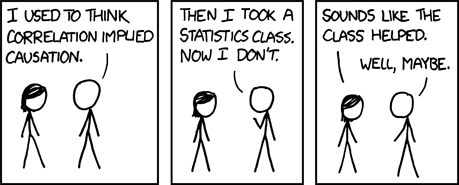
\includegraphics[width=12cm]{correlation.png}
%\end{center}

\newpage
\thispagestyle{empty}

\subsubsection*{Optimal control part}

\begin{enumerate}[resume]

\item	Find extremals that provide the highest or lowest values of the following integral

\[
J(y)=\int _{1}^{e} \left[ \frac{1}{2} x(y')^{2} +\frac{2yy'}{x} -\frac{y^{2} }{x^{2} } \right] \, dx
\]

with the boundary values $y(1)=1$, $y(e)=2$.

\begin{enumerate}
\item (10 points) Find the extremal(s).

\item (10 points) Let $\tilde{y}(x)$ be the extremal you have found. Let  $h(x)\in C^{1} $ and $h(1)=h(e)=0$ ($h(x)$ is not identically zero). Prove that $J(\tilde{y}+h)-J(\tilde{y})>0$.
\end{enumerate}

\item Consider Ramsey's model. Maximize the integral $I=\int _{0}^{\infty }[u(c)-B]dt $ subject to $\dot{k}=f(k)-c-\delta k$, $k(0)=k_{0}$. Function $u(c)$ monotonically increases and tends to $B$ at the infinity, moreover $I$ converges.

\begin{enumerate}
\item (5 points) Derive Ramsey's Law $\frac{d}{dt} u'(c)=u'(c)[\delta -f'(k)]$.

\item (5 points) Let
\[
u(c) =
\begin{cases}
2c - \frac{c^2}{B}, \text{ for } c \leq B \\
B, \text{ otherwise }
\end{cases}
\]
Production function $f(k)=\alpha k$ and $\alpha >\delta $. Find the optimal solutions $c^*,k^*$. Do these solutions necessarily have an economic sense?
\end{enumerate}



\item (10 points) Solve the problem on the bounded optimal control $\int _{0}^{T}(1-\beta -u)xdt \to \max$, subject to $\dot{x}=\alpha xu$, $x(0)=x_{0}$, $0\le u\le 1$. In this problem $\alpha>0$ and $0<\beta <1$.



\end{enumerate}

\end{document}
